% 第三章 基于YOLO的目标检测

\chapter{基于YOLO的目标检测}

\section{卷积神经网络介绍}
卷积神经网络(convolutional neural network, CNN)\cite{lecun1989}是一种专门用来处理具有类似网格结构的数据(如图像)的神经网络\cite{Goodfellow-et-al-2016}。其模拟了生物视觉神经的结构,对传统的神经网络做了一定的改变:将相邻两层神经元之间的全连接改为局部连接,并且同一层内的神经元共享权值。这些改变大大减少了神经网络的参数数量,降低了模型的复杂度,使得网络变得更容易训练。这种网络结构能够直接使用图像作为网络输入,避免了传统算法中人工提取特征的过程,在目标识别、图像分割、目标分类等很多任务中表现突出,得到了学术界与工业界的广泛关注和研究,已被大量应用于计算机视觉的各个领域中。


%\subsection{人工神经网络}
%\subsection{深度学习}
%\subsection{卷积神经网络的历史}

%------------------------------------------------------------------------------------
\subsection{卷积运算及其基本思想}
\subsubsection{卷积运算}
% ref: 吴文正,ch2.3.1,p18
数学上卷积运算包括连续卷积运算和离散卷积运算,它们的定义分别为:
%
\begin{equation}\label{eq:3_1_0}
y(t) = (x*w)(t) = \int_{-\infty}^{\infty}x(a)w(t-a)da
\end{equation}
\begin{equation}
y(n) = (x*w)(n) = \sum_{-\infty}^{\infty}x(i)h(n-i)
\end{equation}
其中的参数$x$是输入,参数$w$被称为核函数(kernel function)。星号表示卷积运算。注意到公式中将核函数进行了翻转,即当输入x的索引增大时,核w的索引是在减小的。通过翻转,卷积获得了可交换的性质,即$x*w=w*x$。

卷积神经网络中的卷积操作是对二维数组进行的,因此是二维离散卷积。而与常规的卷积不同的是,卷积神经网络的卷积计算中并没有进行翻转:
%
\begin{equation}
S(i,j) = (I*K)(i,j) = \sum\limits_{m} \sum\limits_{n} I(i+m,j+n)K(m,n)
\end{equation}
这种计算也被称为互相关函数(cross correlation),卷积核也被称为滤波器(filter)。

%------------------------------------------------------------------------------------
\subsubsection{卷积运算的基本思想}
% DL book, ch9.2, p313.
% 何鹏举,ch2.2,p16; 黄咨,ch3.3,p48.
% http://blog.csdn.net/zlrai5895/article/details/78634800?locationNum=6&fps=1
神经网络在过去几十年经历了多次起起落落,是因为其应用存在着很多困难。当网络较浅时,其无法刻画复杂的非线性关系,因此对于较多的数据和复杂的模式,无法得到理想的分类或预测性能;而如果网络很深或求解问题规模较大,则网络内的参数数量会急剧增加,运算量也会成指数级增长,导致训练无法完成。
卷积神经网络将卷积运算引入神经网络,而卷积运算包含了三个改进神经网络算法的重要思想:稀疏连接、参数共享和等变表示。

(1) 稀疏连接(局部感知)

传统神经网络使用矩阵乘法来建立各层网络的输入与输出之间的关系。参数矩阵中的每个元素都描述了上一层网络中某个神经元的输出与下一层网络的某个神经元的输入之间的交互,即每个输出单元与每个输入单元都存在着联系。然而,卷积网络具有稀疏连接的特点。输入图像中可能包含几万甚至几百万的像素点,但并没有必要让每个神经元都对整幅图像进行感知,因为局部区域内的像素联系比较大,而距离远的像素之间通常并没有很强的相关性。
使用只包含几十到几百个像素的小尺寸的卷积核,就可以检测图像中局部的特征,如边缘等。稀疏连接可以大大减少模型中的参数数量。

局部连接虽然使得每个神经元只与其前一层中很少的神经元有联系,但由于卷积神经网络有多层,通过层层的传递,处于网络中更深层的神经元实际上与相当多的浅层神经元之间存在着联系,它们比处在浅层的神经元具有更大的接受域。也就是说,深层的神经元将浅层神经元中的局部信息逐渐综合起来,从而得到了全局信息。这种模式非常类似于人类由局部到全局的视觉感知过程,因此稀疏连接的特性也被称为局部感知。

\begin{figure}[htb] %稀疏连接与全连接的对比;更深层的神经元具有更大的接受域
	\centering
	\begin{minipage}[c]{0.48\textwidth}
		\centering
		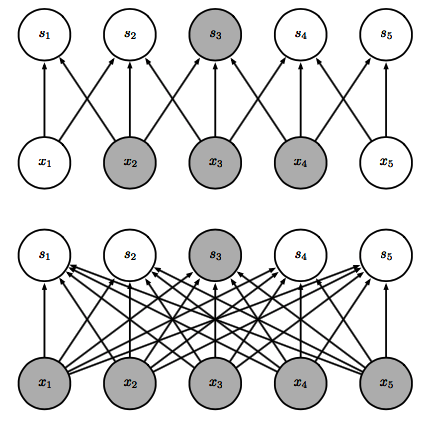
\includegraphics[width=3in]{figures/3_1_稀疏连接与全连接的对比}
		\caption{稀疏连接与全连接的对比}
	\end{minipage}
	\hfill
	\begin{minipage}[c]{0.48\textwidth}
		\centering
		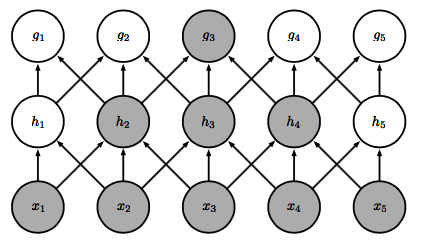
\includegraphics[width=3in]{figures/3_1_更深层的神经元具有更大的接受域}
		\caption{更深层的神经元具有更大的接受域}
	\end{minipage}
\end{figure}

(2)参数共享

参数共享是指对于不同的神经元使用相同的权重参数。在传统神经网络中,每层网络的权重矩阵W中的元素都仅仅被使用了一次,这是非常低效的。而在卷积神经网络中,卷积层通过平移卷积核遍历了整个特征平面,也就是说每个卷积核内的参数都是在这一整层网络中共享的。卷积参数的共享使得我们不需要区别对待每个位置,只要学习一个参数集合即可。事实上,对卷积核参数的学习可以理解为对特征提取方式的学习,该方式是与位置无关的。比如当一个卷积核能用来提取沿某个方向的梯度特征时,使用该卷积核能在整个特征平面上提取到所有沿该方向的梯度特征。与稀疏连接类似,参数共享也能够显著降低网络模型中的参数数量。

\begin{figure}[htb] %卷积运算的参数共享
	\centering
	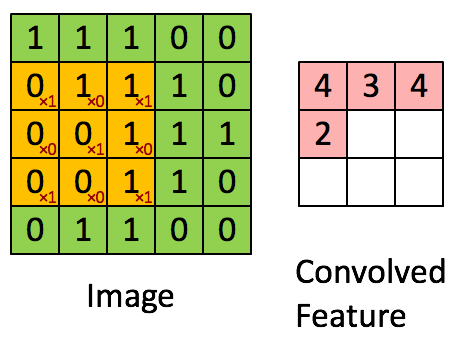
\includegraphics[width=3in]{figures/3_1_参数共享1}
	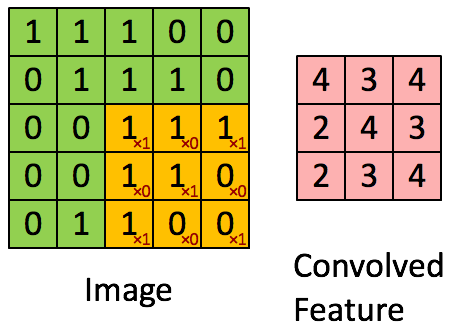
\includegraphics[width=3in]{figures/3_1_参数共享2}
	\caption{卷积核的参数共享} \label{fig:3_1_卷积核的参数共享}
\end{figure}

需要说明的是,一个二维的卷积核只能提取某种特定的特征,而图像中含有多种特征,显然只提取一种特征是非常不充分的。因此卷积层的输入输出一般是多个特征图堆叠起来的3维特征卷(feature volume),此时对应每个输出特征图的卷积核是3维的,或者认为是多个2维的卷积核,每个作用于输入特征卷中的一个特征图,则这些2维的卷积核之间是不共享参数的,如图所示\ref{fig:3_1_三维卷积核}。

\begin{figure}[htb] %三维卷积核
	\centering
	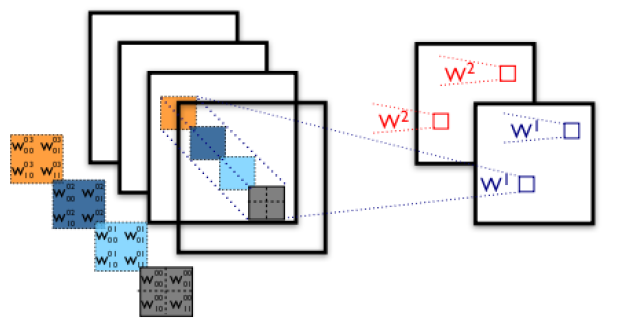
\includegraphics[width=4in]{figures/3_1_三维卷积核}
	\caption{三维卷积核} \label{fig:3_1_三维卷积核}
\end{figure}

%如图\ref{fig:3_1_卷积核的参数共享},输入图像的尺寸是5*5,使用大小为3*3的卷积核来提取图像中的特征,仅需要9个参数。而如果不共享卷积核的参数,则输出的特征图上的每个元素都需要9个参数,输出共有9个元素,故该卷积层需要9*9=81个参数。实际中的图像尺寸远大于9*9,但无论图像多大,卷积核都可以使用3*3的尺寸,则参数共享减少的网络参数数量会更为显著。

我们使用一个具体的例子来定量地分析一下稀疏连接和参数共享在减少网络模型参数数量方面的作用。对于一张尺寸为1000 * 1000的灰度图像,假设输出10个尺寸为500 * 500的特征图,当使用全连接时,该层网络参数共有1000 * 1000 * 500 * 500 * 10 = 2.5e12,如果每个参数占4字节,那么仅保存这些参数就需要9313G的空间,显然这么多的参数是无法训练的。而如果使用尺寸为3*3的卷积核,仅使用稀疏连接时,该层所需参数数量为500 * 500 * 3 * 3 * 10 = 2.25e6,相比2.5e12减小了6个数量级。再加入参数共享,则只需要3 * 3 * 10 = 90个参数。可见,稀疏连接和参数共享在减少网络模型参数数量上的作用是十分惊人的。

(3)等变表示

参数共享使得卷积层具有对平移等变(equivariance)的性质。
函数的等变性指的是函数的输入与输出以相同的方式发生改变,而卷积对平移等变也就是说,对于一张特征图,先对其进行卷积,然后对卷积结果进行平移,与先进行平移再应用卷积的效果是一样的。这也就说明了参数共享能使卷积操作对于整个特征图中的各个位置发挥相同的作用,因而一个特定的卷积核能用于提取散落在特征图中各处的相同特征。卷积对于缩放或旋转等变换并不具有等变性,但通过一些其他机制可以使其具有等变性。
比如,将旋转角度离散化,用多个卷积核各对应一个角度,则当输入旋转某个角度时,总会有一个过滤器被激活,则再使用一个最大池化单元,即可获得对旋转变换的不变性。

%------------------------------------------------------------------------------------
\subsection{卷积神经网络结构}
% ref: 吴正文,ch2.2,p18; 何鹏举,ch2.3,p19; 陈拓,ch3.1.3,p36.
卷积神经网络将传统神经网络的全连接层改为了卷积层,因此其基本网络结构一般包含输入层、卷积层、下采样层和输出层几个部分,有些网络仍然包含全连接层,如图\ref{fig:3_1_卷积神经网络结构}所示。

\begin{figure}[htb] %卷积神经网络结构
	\centering
	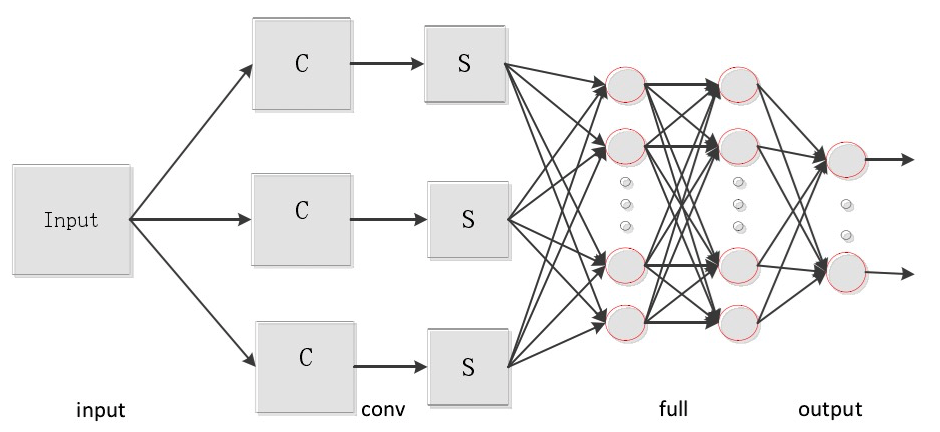
\includegraphics[width=4in]{figures/3_1_卷积神经网络结构}
	\caption{卷积神经网络结构} \label{fig:3_1_卷积神经网络结构}
\end{figure}

输入层:输入层的输入一般为经过某些预处理后的图像,预处理包括灰度化、像素值归一化、裁剪和调整为特定尺寸等。如果把处理后的图像也视为特征图的话,则对于灰度图,输入层为单个特征图,对于彩色图像,输入层为多个特征图,每个对应图像的一个通道。

卷积层:卷积层是卷积神经网络的核心组成部分,其作用是提取图像中的特征,因此也被称为特征提取层。通常卷积层中会使用多个卷积核以提取不同类型的特征,基于每个卷积核可以得到一个特征图(或叫特征平面),故卷积层的输入和输出都是多个特征图堆叠形成的特征卷。卷积层的每个神经元从前一层的局部感受野中提取某种特征,接近输入层的卷积层提取的特征较为低级,在经过多个卷积层之后,特征会逐渐变得更高级、更抽象,同时也会包含更大范围的信息。在对输入的特征图进行卷积运算后,还要像传统神经网络一样加入偏置项(bias),并经过某种类型的非线性激活函数以获得非线性的拟合能力:
%
\begin{equation}
y_l = f(W*y_{l-1}+b)
\end{equation}
$f(\cdot)$表示激活函数。激活函数通常具有非线性、可微性、单调性的性质,常见的激活函数有sigmoid, tanh, 整流线性单元(ReLU)等。sigmoid能把实数范围内的输入压缩到0到1之间输出,但它有一个严重的缺点,当输入非常大或非常小时,函数会饱和,梯度趋向于0,无法实现有效的梯度下降。tanh是sigmoid的变形,tanh(x) = 2sigmoid(2x) - 1,它通常比sigmoid的表现更好,因为其均值为零。整流线性单元不存在饱和的问题,当其处于激活状态时,一阶导数处处为1,因此它的梯度方向效率较高。但它的问题是一旦取值为零,则它的梯度永远为零,也就无法再次激活了,可以认为这个神经元“死亡”了。当设置的学习率较大时,网络中会有大量的神经元死亡。为了解决这个问题,出现了一些ReLU的变种,比如渗透整流线性单元(leaky ReLU)\cite{maas2013rectifier},其定义为f(x,a)=max(0,x)+a*min(x,0),a一般取为类似0.01的小值。
% leaky relu的介绍
\begin{figure}[htb] %激活函数
	\centering
	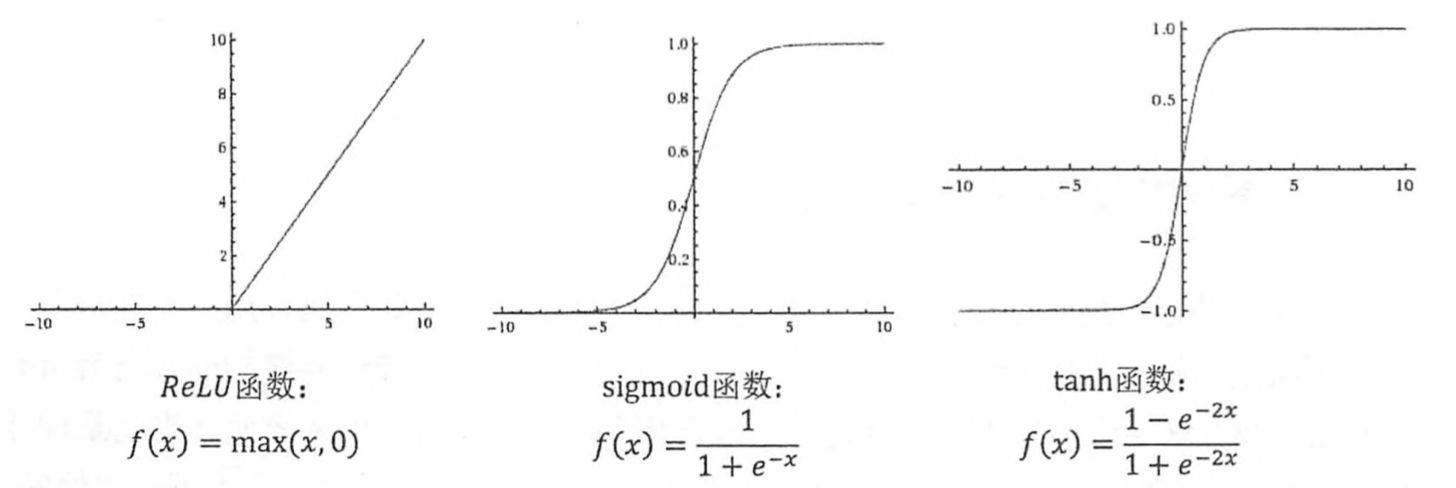
\includegraphics[width=4in]{figures/3_1_激活函数}
	\caption{激活函数} \label{fig:3_1_激活函数}
\end{figure}

每个卷积层的输出尺寸由输入特征图尺寸、卷积核尺寸、步长和边界处的零填充(zero padding)等参数共同决定。设输入、输出特征图分别为边长$x_{i}$和$x_{o}$的正方形,卷积核为边长k的正方形,卷积运算的步长为stride,零填充个数为pad,则输出特征图的尺寸可根据下式来计算:
%
\begin{equation}
x_o = \frac{x_i + 2 \times pad - k}{stride} + 1
\end{equation}


下采样层:下采样层也称为子采样层或池化层,该层的引入是为了在保留有用信息的同时尽量减小数据的维度,本质是一种聚合的操作。下采样的核心是池化函数,它决定了用某一位置所在矩形邻域内的哪一种统计特征作为该位置的输出。池化函数可以表示为:
\begin{equation}
O = (\sum \sum I(i,j)^P \times G(i,j))^{1/P}
\end{equation}
其中,I和O分别表示池化层的输入、输出特征图,G表示高斯核函数,P在$[1, \infty)$内取值。当P=1时,池化被称为平均池化,取各个子区域内元素的均值作为输出;而当$P\rightarrow \infty$时,使用的是最大池化,即输出每个子区域内的最大元素。
如果池化层的输入特征图尺寸为m*n,池化操作水平和竖直方向的步长为w和h,则下采样后输出的特征图尺寸为(m/w)*(n/h)。最常见的采样块尺寸为2*2。
池化操作除了能够降低参数数量外,也能够有效地防止过拟合现象的发生。此外,池化操作还能使卷积层的输出获得局部平移不变性的性质,也就是说,当对该层的输入进行微小的平移时,池化后该层的大多数输出都不会变化。
该性质很重要,因为我们通常只关心某个特征是否出现,而并不关心它的具体位置。

\begin{figure}[htb] %最大池化和平均池化
	\centering
	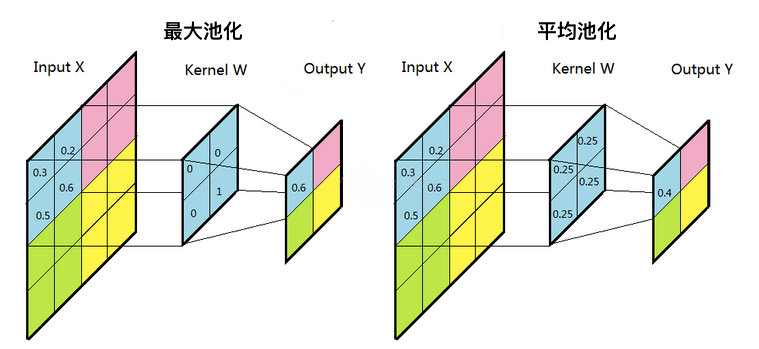
\includegraphics[width=4in]{figures/3_1_最大池化和平均池化}
	\caption{最大池化和平均池化} \label{fig:3_1_最大池化和平均池化}
\end{figure}
%此外,在卷积层中设置卷积的步长和零填充也可以实现下采样的功能。

全连接层:全连接层通常位于最后一个卷积或采样层与输出层之间,用于将二维特征图转变为一维特征向量。全连接层的每个神经元与前一层的每个神经元相连,因此相当于两个矩阵相乘。使用全连接层会给卷积神经网络带来一些限制,因为卷积操作使得卷积层可以接受任意尺寸的输入,而全连接层的神经元个数固定,因此图像尺寸不能随意改变,当输入不同尺寸的图像时,可能需要首先进行缩放或裁剪的处理。

输出层:输出层的设计基于网络的具体应用任务。比如对于图像识别,输出层通常会是一个分类器。常用的分类器包括多项式逻辑回归(Multinomial Logistic Regression)分类器、softmax分类器等,也可以使用一到两层的全连接层作为分类器。
% softmax分类器介绍: 何鹏程, ch2.3.3, p21.

%------------------------------------------------------------------------------------
\subsection{卷积神经网络的训练}
% SGD,反向传播算法;损失函数;正则化。学习率。
\subsubsection{反向传播算法}
% 这块太蛋疼了。。凑活一下吧。。
卷积神经网络的训练与传统人工神经网络的训练类似,主要可以分为有监督、无监督和二者结合等几种方式。本文使用的模型都基于有监督学习,即网络利用带标记的训练样本数据进行学习,训练数据的标记即为监督信号。卷积神经网络的训练本质上是一个优化问题,即定义一个目标函数并将其最小化,该函数也称为代价函数或损失函数。训练常使用基于梯度的方法,主要包括前向传播和反向传播两个阶段。
前向传播即由网络输入经过层层的卷积、池化等操作后求得网络输出的过程,比较简单;反向传播是指由网络的输出值与训练数据的真值之间的误差反向逐层计算各层权重与偏置项的梯度,并根据学习率来更新这些参数使损失函数值逐渐下降至最终收敛。下面简要介绍一下反向传播的计算\cite{bouvrie2006notes}。

% 实在是没有精力看论文推公式了,先抄一下。。
% <Notes on Convolutional Neural Networks>, http://cogprints.org/5869/1/cnn_tutorial.pdf
% http://www.hankcs.com/ml/sgd-cnn.html  (a,z是啥没说明就出现在公式里,看不懂,不用了)
% http://deeplearning.stanford.edu/wiki/index.php/反向传导算法
(1)全连接层的反向传播

令$l$表示当前层,输入层和输出层编号分别为$1$和$L$。定义当前层的输出为$x^l = f(u^l)$,其中$u^l = W^l x^{l-1} + b^l$,$f(\cdot)$表示激活函数。则由下一层传到当前层的残差为:
\begin{equation}\label{eq:3_1_残差_全连接层}
\delta^{l} = ((W^{l+1})^T \delta^{l+1} ) \circ f'(u^l)
\end{equation}
式中$\circ$表示逐元素的乘法。损失函数关于当前层的权重W和偏置b的梯度为:
%% align环境占两行太浪费了,一行挤一挤就好
%\begin{align}
%\frac{\partial E}{\partial W^l} &= x^{l-1}( \delta^l )^T \label{eq:3_1_w梯度_全连接层} \\
%\frac{\partial E}{\partial b^l}  &= \delta^l \label{eq:3_1_b梯度_全连接层}
%\end{align}
\begin{equation}
\frac{\partial E}{\partial W^l} = x^{l-1}( \delta^l )^T, \quad
\frac{\partial E}{\partial b^l}  = \delta^l
\end{equation}


(2)卷积层的反向传播

在卷积层中,每个输出的特征图结合了多个输入特征图的卷积结果。将当前层的输出表示为:
\begin{equation}
x_j^l = f \left( \sum\limits_{i \in M_j} x_i^{l-1} * k_{ij}^l + b_j^l \right)
\end{equation}
式中$M_j$表示输入特征图中的某一个。假设每个卷积层$l$后面都有一个下采样层$l+1$,下采样层中的权重都为$\beta$,则计算残差为:
\begin{equation}
\delta_j^l = \beta_j^{l+1} (f'(u_j^l) \circ up(\delta_j^{l+1})) \label{eq:3_1_残差_卷积层}
\end{equation}
其中$up(\cdot)$表示上采样操作,如果下采样的因子为n,则上采样将每个元素沿水平和竖直方向重复n次。进而可以计算损失关于偏置和卷积核权重的梯度:
%\begin{align}
%\frac{\partial E}{\partial k_{ij}^l} &= \sum\limits_{u,v} (\delta_j^l)_{uv} (p_i^{l-1})_{uv} \label{eq:3_1_w梯度_卷积层} \\
%\frac{\partial E}{\partial b^j}  &= \sum\limits_{u,v} (\delta_j^l)_{uv} \label{eq:3_1_b梯度_卷积层}
%\end{align}
\begin{equation}
\frac{\partial E}{\partial k_{ij}^l} = \sum\limits_{u,v} (\delta_j^l)_{uv} (p_i^{l-1})_{uv} , \quad
\frac{\partial E}{\partial b^j}  = \sum\limits_{u,v} (\delta_j^l)_{uv}
\end{equation}
$(p_i^{l-1})_{uv}$是$x_i^{l-1}$中与卷积核$k_{ij}^l$逐元素相乘的小块。使用MATLAB语句的表示更直观:
\begin{equation}
\frac{\partial E}{\partial k_{ij}^l} = rot180(conv2(x_i^{l-1}, rot180(\delta_j^l), 'valid'))
\end{equation}
'valid'表示卷积的填充方式,旋转180度是为了使用卷积函数来进行互相关操作。

(2)下采样层的反向传播

下采样层的输出表示为:
\begin{equation}
x_j^l = f \left( \beta_j^l down(x_j^{l-1}) + b_j^l \right)
\end{equation}
$down(\cdot)$表示下采样函数。则残差可使用下面的语句求取:
\begin{equation}
\delta_j^l = f'(u_j^l) \circ conv2(\delta_j^{l+1}, rot180(k_j^{l+1}, 'full'))
\end{equation}
定义$d_j^l = down(x_j^{l-1})$,则损失函数关于$b$和$\beta$的梯度分别为:
%\begin{align}
%\frac{\partial E}{\partial b^j}  &= \sum\limits_{u,v} (\delta_j^l)_{uv} \\
%\frac{\partial E}{\partial \beta^j} &= \sum\limits_{u,v} (\delta_j^l \circ d_j^l)_{uv}
%\end{align}
\begin{equation}
\frac{\partial E}{\partial b^j}  = \sum\limits_{u,v} (\delta_j^l)_{uv} , \quad
\frac{\partial E}{\partial \beta^j} = \sum\limits_{u,v} (\delta_j^l \circ d_j^l)_{uv}
\end{equation}

\subsubsection{随机梯度下降}
% SGD, DL book, ch5.10, p160.
% http://www.hankcs.com/ml/sgd-cnn.html
传统梯度下降使用的损失函数通常是对每个输入样本的代价的累积。对于使用n个样本的模型来说,计算每一个梯度的运算代价为O(n)。而深度神经网络的训练需要大量的样本数据,训练集规模可能为上亿的量级,而且模型中的参数也非常多,因此这种计算梯度的策略运算量巨大,非常耗时;另外由于计算机的内存和显存有限,一次性载入大量的训练数据也是不现实的。在这种背景下,随机梯度下降(stochastic gradient descent,SGD)算法应运而生。随机梯度下降的核心思想是,把梯度作为期望来对待,即使用一小部分的样本数据来做一个近似估计。对于训练的每一次迭代,仅从整个训练数据集中抽取很小的一批(minibatch)样本数据用于训练。这个小批量数据的个数m一般取值为1到几百,不论整个训练集的规模增长到多大,m通常都是不变的。算法\ref{alg:sgd}给出了随机梯度下降的具体步骤。
% DL book,ch8.3.1,p279.
\begin{algorithm}[htb]
	\caption{随机梯度下降在第$k$个训练迭代的更新}
	\label{alg:sgd}
	\begin{algorithmic}
		\REQUIRE 学习率 $\epsilon_k$
		\REQUIRE 初始参数$\theta$
		\WHILE{终止训练条件未满足}
		\STATE 从训练数据集中取出$m$个样本$\{ x^{(1)},\dots, x^{(m)}\}$ ,其中$x^{(i)}$对应目标为$y^{(i)}$。
		\STATE 计算梯度的估计值: $\hat{g} \leftarrow + 
		\frac{1}{m} \nabla_{\theta} \sum_i E(f(x^{(i)};\theta),y^{(i)})$
		\STATE 更新参数:$\theta \leftarrow \theta - \epsilon \hat{g}$
		\ENDWHILE
	\end{algorithmic}
\end{algorithm}

学习率是随机梯度下降中的一个很重要的参数。随机梯度下降使用的学习率比普通梯度下降的学习率要小很多,因为其梯度变动比较剧烈,方差较大。在实践中一般要随着迭代次数的增加而逐渐降低学习率,比如可以使用线性衰减的学习率,或者每隔一段时间将学习率减半。更好的方法是预留一部分数据用于每次迭代完成后计算目标函数的输出值,当相邻两次迭代输出的变化小于某个阈值时才减小学习率。一般获取每个批之前要将数据随机打乱,否则得到的梯度可能偏离正确的方向,导致收敛性差。

另外还有很多针对梯度下降的优化算法,如动量法、Adagrad、RMSprop、自适应矩估计(Adam)等,在此不再详细介绍。

\subsubsection{正则化}
% DLbook,ch5.2.2,p132; ch7,p225(L1, L2).
一般我们在训练集之外会使用一个测试集来检验模型的泛化能力,而模型经常会出现欠拟合和过拟合的问题。欠拟合指模型在训练集上不能获得理想的效果,而过拟合指模型在训练集上表现良好,但在测试集上表现很差,训练误差和测试误差之间存在较大的差距。通过调整模型的容量,也就是模型可以选择的函数的数目,可以控制模型对于这两种问题的倾向。根据统计学习理论,随着模型容量变大,训练与泛化误差之差的上界会逐渐增大,因此通过限制模型容量可以改善过拟合现象。

\begin{figure}[htb] %欠拟合和过拟合
	\centering
	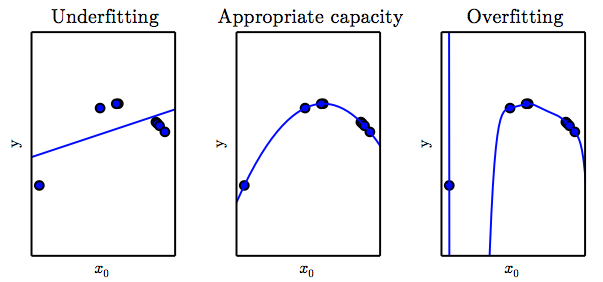
\includegraphics[width=3.5in]{figures/3_1_欠拟合和过拟合}
	\caption{欠拟合和过拟合现象} \label{fig:3_1_欠拟合和过拟合}
\end{figure}

正则化就是用来降低泛化误差、改善过拟合现象的策略。最常见的操作是,在目标函数中加入参数范数的惩罚,从而限制模型参数的增长。对于神经网络中的参数,一般只对权重参数W做惩罚,而不考虑偏置参数b。常用的参数范数惩罚包括L2正则化和L1正则化,分别在目标函数中加入权重的2-范数和1-范数作为惩罚。


%------------------------------------------------------------------------------------

\section{YOLO目标检测模型}
% YOLO paper; 
% 杨眷玉《基于卷积神经网络的物体识别研究与实现》; 
% 郑嘉祺《基于DCNN的井下行人检测系统的研究与设计》.
YOLO(You Only Look Once)\cite{redmon2016you}是一种实时性非常好的基于卷积神经网络的目标检测模型,它的运行速度可以达到45帧/秒,而其简化版本甚至可以达到150帧/秒以上,非常适合于在实时性方面有较严格的要求的应用场景。

YOLO模型之所以能够实现如此高的运行速度,主要是因为在对目标检测任务进行建模时使用了一种新颖的思路,将目标检测作为一个回归问题来处理。其他主流的目标检测算法,如可变形部件模型(DPM)和基于卷积神经网络的R-CNN系列,大都将目标检测作为一个分类问题来处理,首先需要使用滑动窗口、区域提名(region proposal)等方法初步生成一系列可能包含待检测物体的检测框,再使用分类器来判断每个检测框中包含哪种物体,完成后还要进行很多后处理来改善结果,过程繁琐,耗时较大。

与此相对,YOLO的训练和检测完全基于一个单独的网络,它直接建立输入图像像素与检测框坐标和目标属于某个类别的概率之间的回归关系。因此,这个模型只需要一次性提取图像信息后即可预测图像中存在的全部物体及其具体位置,这也是模型被命名为“You Only Look Once”的原因。
基于其简单的网络结构,YOLO在整幅图像上进行训练,并能够直接根据训练数据来改善其检测的性能。
由于能够利用整张图像的全局信息来对每个检测框进行预测,YOLO不易发生对背景的误检,在获得优秀的运行效率的同时也保证了较高的检测精确度。

%------------------------------------------------------------------------------------
\subsection{目标检测策略与过程}
YOLO将每幅待检测图像分割为$S\times S$个方格(grid),图像中每个物体的中心部分所在的小方格负责该物体的检测,如图\ref{fig:3_2_物体中心所在方格负责检测该物体}所示,图中狗所在边界框的中心位于坐标为(5,2)的方格中,因此该方格负责检测该图中的狗。每个单元格要预测$B$个边界框(bounding box),并为每个边界框给出一个置信度,这个置信度既要反映单元格对于包含所要检测的物体的信心,也要体现单元格对于该检测框的位置和尺寸的准确度的把握,因此可以定义为:
\begin{equation}
Confidence = P(Object) \times IOU_{pred}^{truth}
\end{equation}
其中,$P(object)$用于描述第一个因素。如果单元格认为自己负责的范围内并没有待检测的物体,则P = 0,从而置信度也就为0。而如果单元格认为自己是包含某种目标物体的,则P = 1,从而Confidence = IOU。IOU就是用来描述第二个因素的,即单元格对检测框的位置准确性的信心。IOU全称为Intersection Over Union,某些文献内翻译为“交并比”,因为它的定义是模型预测的检测框Pred与训练数据中标记的准确包含该物体的边界框Truth的交集与并集的比值:
\begin{equation}
IOU_{pred}^{truth} = \frac{Pred \cap Truth}{Pred \cup Truth}
\end{equation}
图\ref{fig:3_2_IOU}给出了更直观的IOU的概念。IOU体现了检测框与真实边界框的重合度,我们希望重合度尽可能的高,如果两个矩形框完全重合则IOU为1,也就达到了最理想的效果。

\begin{figure}[htb] %物体中心所在方格负责检测该物体; IOU
	\centering
	\begin{minipage}[c]{0.48\textwidth}
		\centering
		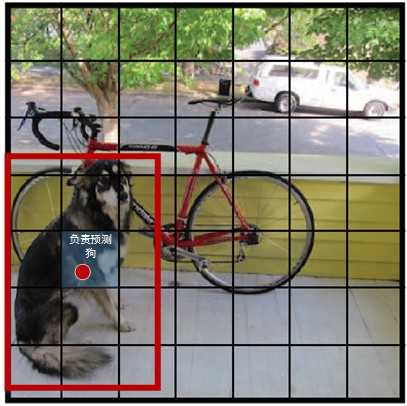
\includegraphics[width=2in]{figures/3_2_物体中心所在方格负责检测该物体}
		\caption{物体中心所在方格负责检测该物体} \label{fig:3_2_物体中心所在方格负责检测该物体}
	\end{minipage}
	\hfill
	\begin{minipage}[c]{0.48\textwidth}
		\centering
		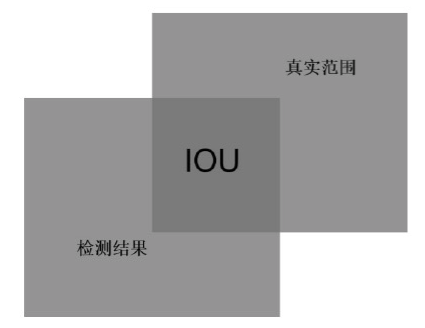
\includegraphics[width=2.5in]{figures/3_2_IOU}
		\caption{IOU示意图} \label{fig:3_2_IOU}
	\end{minipage}
\end{figure}

对于每个检测框有五个需要预测的参数,包括检测框的中心点坐标(x, y),检测框的宽度w和高度h,以及上面定义的置信度Confidence。检测框的中心点坐标(x, y)是相对于其所在小方格的偏移量,并以方格的边长为基准归一化到[0, 1]之间;而其宽度和高度则是以图像尺寸的宽度和高度来归一化到[0, 1]区间的。

在与每个检测框相关的5个参数之外,对于每个小方格,还需要预测C个物体类别的条件概率$P(Class_i|Object)$,C为模型能够预测的类别的数目。根据该条件概率的表示方式可知,其前提条件是小方格内包含某种物体。无论每个小方格中要预测的检测框的数量B是多少,我们只对每个小方格预测一组各个类别的条件概率。这样,在进行预测时,使用某个方格内每个物体类别的条件概率乘以该方格内每个检测框的置信度,即可得到每个检测框包含每种类别物体的置信度分数:
\begin{equation}
P(Class_i | Object) * P(Object) * IOU_{pred}^{truth} = P(Class) * IOU_{pred}^{truth}
\end{equation}
由上式可见,最终的置信度得分既反映了检测框包含某种待检测物体的概率,也反映了检测框定位该物体的效果,即检测框的位置与尺寸的精确程度。

% 检测流程
YOLO模型进行物体检测的具体过程如图\ref{fig:3_2_YOLO检测过程}所示。整个过程可以分为三个阶段:首先将输入图片缩放到网络的固定输入尺寸,即边长为448的正方形;之后进行卷积神经网络的前向传播过程,求取每个检测框包含每种物体的概率及检测框的位置,根据一个概率阈值来筛除置信度比较低的结果;最后利用非极大值抑制算法进一步筛除冗余的检测框,将精确度最高的结果作为最终检测结果输出。

\begin{figure}[htb] %YOLO检测过程
	\centering
	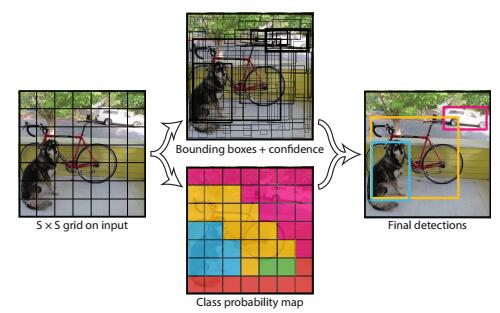
\includegraphics[width=5in]{figures/3_2_YOLO检测过程}
	\caption{YOLO检测过程} \label{fig:3_2_YOLO检测过程}
\end{figure}

%NMS
非极大值抑制(Non Maximum Suppression, NMS)算法是一种获取局部极大值的方法,在目标检测中经常被用来筛除冗余的候选框。该算法的具体步骤是,首先根据各个候选框的得分进行排序,然后以得分最高的候选框为基准,依次计算其余候选框与基准候选框的IOU,若IOU大于一定的阈值,则删除此候选框(将其得分改为0);再从剩余候选框中选择得分次高的候选框作为基准,遍历得分小于它的候选框并根据IOU来决定是否删除,重复此过程,直至最终任意两个候选框的IOU都小于所设定的阈值。非极大值抑制的效果如图\ref{fig:3_2_NMS}所示。

\begin{figure}[htb] %非极大值抑制
	\centering
	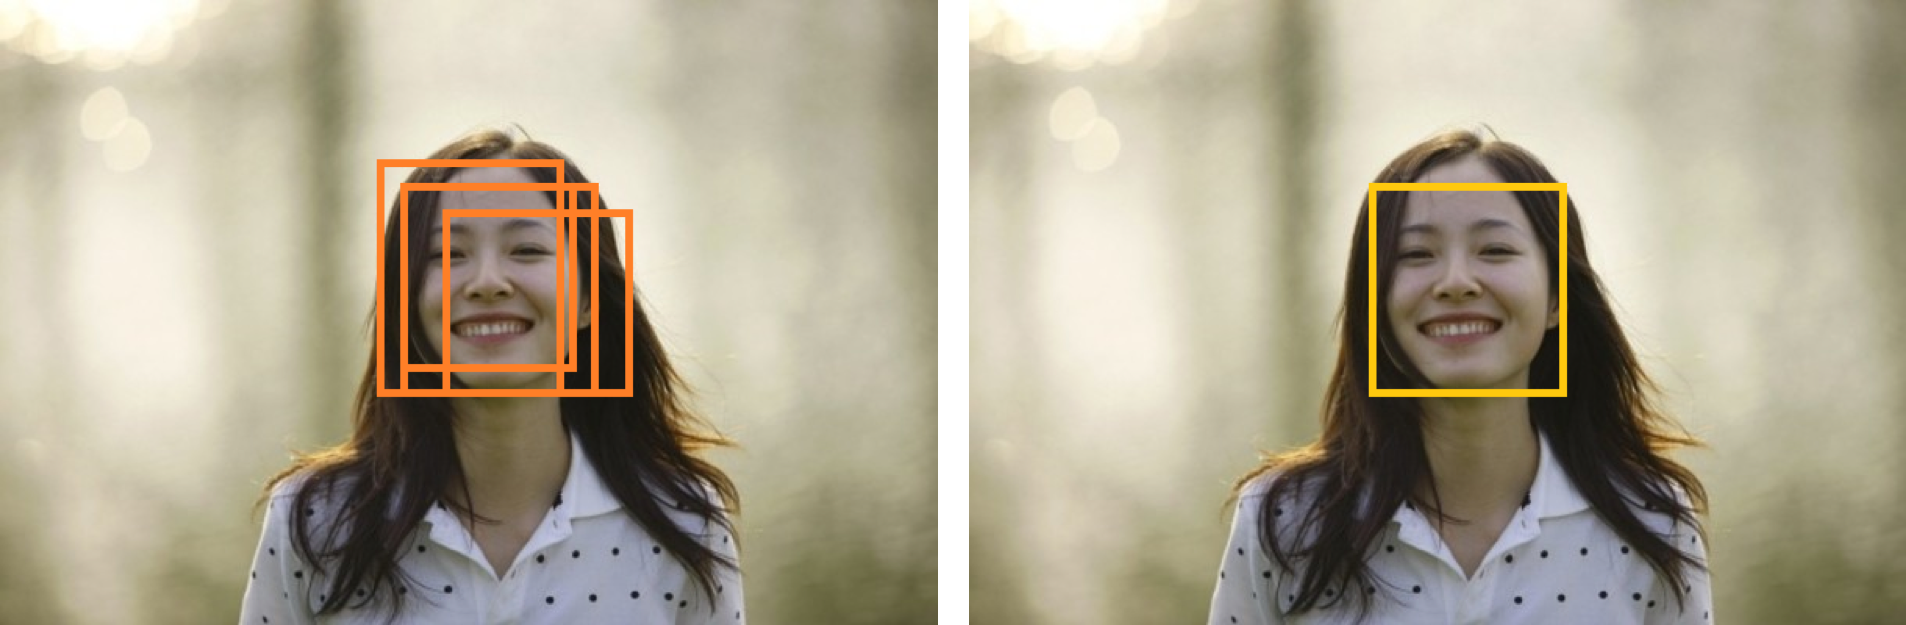
\includegraphics[width=5in]{figures/3_2_NMS}
	\caption{非极大值抑制} \label{fig:3_2_NMS}
\end{figure}

%------------------------------------------------------------------------------------
\subsection{网络结构}
YOLO的网络架构借鉴了用于图像分类的GoogLeNet\cite{szegedy2015going},其包含24个卷积层和2个全连接层,卷积层负责图像特征的提取,全连接层用来预测检测框的概率和坐标。与GoogLeNet的区别是,YOLO替换掉了结构比较复杂的Inception模块,改用1*1的卷积层实现降维,然后加上一个3*3的卷积层。具体的网络结构如图\ref{fig:3_2_YOLO网络结构}所示。

\begin{figure}[htb] %YOLO网络结构
	\centering
	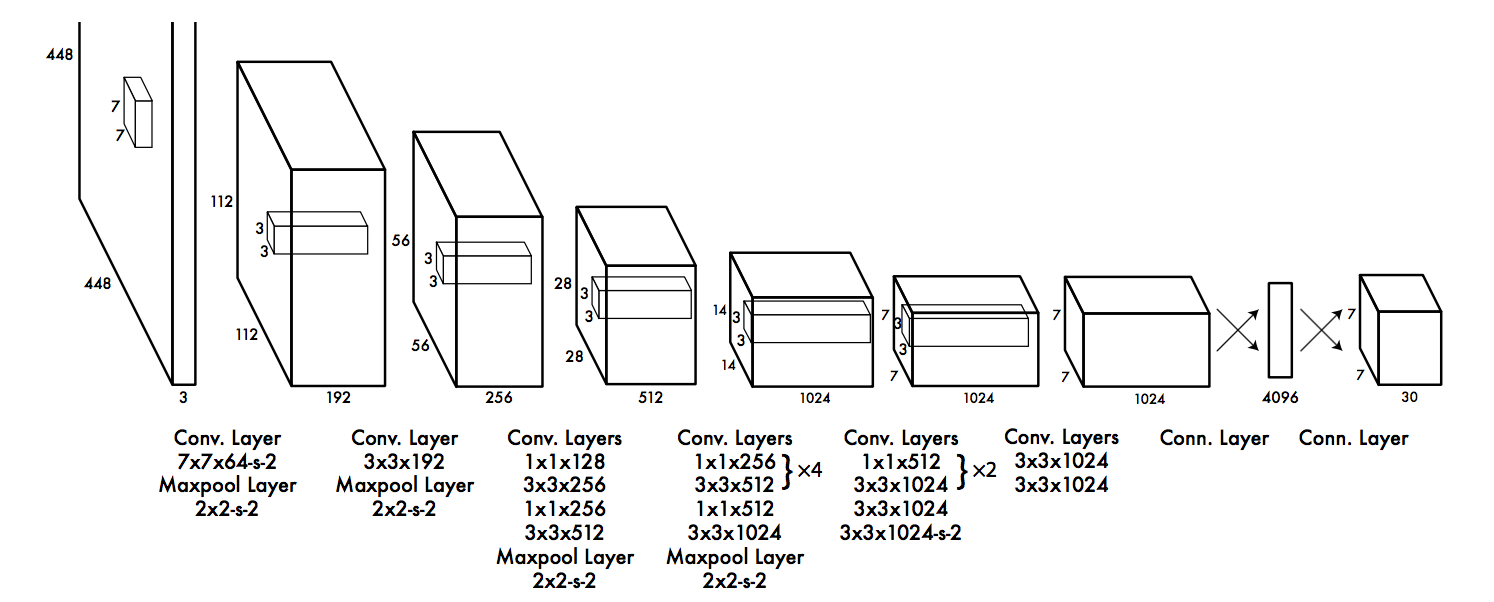
\includegraphics[width=5in]{figures/3_2_YOLO网络结构}
	\caption{YOLO网络结构示意图} \label{fig:3_2_YOLO网络结构}
\end{figure}

根据前面的介绍,每个方格预测B个检测框以及C个类别的条件概率,每个检测框又包含5个参数,因此每个方格共对应B*5 + C个参数。在实际应用中,设置S = 7, B = 2,使用的数据集包含20个物体类别,即C = 20,从而卷积神经网络的预测输出为7 * 7 * (2 * 5 + 20) = 7 * 7 * 30的三维数组。

网络中使用的激活函数为渗透整流线性单元(leaky ReLU)f(x) = max(0, x) + 0.1*min(x, 0),但最后一层使用线性激活函数。另外,在最后一个全连接层之前使用了dropout\cite{hinton2012improving},在训练中随机丢弃50\%的神经元输出。dropout是一类比权重衰减计算开销更小的正则化方法,因为它不需要修改代价函数,而是改变网络本身的结构。只在一层中使用dropout并不会显著减小模型的有效容量,却可以有效地防止过拟合。

另外还有一个简化版本的Fast YOLO网络,仅使用了9个卷积层。 但由于YOLO的实时性能已经可以满足需求,而Fast YOLO的检测精度要略差一些,因此不考虑使用简化版。


\subsection{损失函数的定义} % 及改进}
由于目标检测任务需要预测出图像中物体的类型以及对应检测框的位置和尺寸,YOLO的损失函数包含了四部分内容,分别用来监督检测框的中心坐标、检测框的宽度和高度、每个检测框中是否包含待检测物体的置信度以及检测到的物体属于每种类别的概率。每一项都是误差平方和的形式,因为误差平方和的梯度比较简单,从而损失函数比较容易进行优化。

然而这种将多个损失项简单相加的形式存在诸多的问题,它并不能保证模型在这四个方面达到很好的平衡并最终获得理想的检测准确度。首先,在与每个方格对应的30维向量中,与检测框定位误差(包括位置和尺寸)相关的元素有8个,而与分类误差相关的有20个元素,给这两者的损失项赋予同等的重要性显然是不合理的;另外,在一张图像中,包含待检测物体的方格数量可能会远小于不包含待检测物体的方格数量,从而会有大量方格的置信度得分为零,而只有少量方格有非零的置信度,正负样本的分布非常不均衡,会导致正样本包含的信息在梯度下降中无法正常发挥作用,最终网络的损失函数难以收敛甚至会发散。

为了解决这些问题,我们可以对各个损失项进行加权来调整各项的重要程度。具体地,主动增加检测框坐标误差对应的损失函数权重系数$\lambda_{coord}$,并减小检测框不包含待检测物体时置信度得分的损失函数权重$\lambda_{noobj}$。

另外,针对检测框尺寸误差对应的损失项,使用误差平方和也是存在问题的。对于一个较大的检测框和一个较小的检测框,如果网络对它们的预测宽度的误差值相同,则二者的平方和损失是相同的;但显而易见,该误差对于较小的检测框的影响要远远大于对较大检测框的影响。比如,假设两个检测框宽度分别为10和2,网络对它们的预测误差都为1,则前者只偏离了十分之一,而后者却相差了一半。算法提出者通过改为预测检测框宽度和高度的平方根,在一定程度上改善了这种影响,如图\ref{fig:3_2_检测框尺寸平方根的敏感性曲线}所示,当绝对误差相同时,较大的检测框的平方根误差小于较小的检测框。

% 注意本页的空白。(图如果放在loss公式之前,公式被挤到下一页,前一页可能会有很大空白。)
\begin{figure}[htb] %检测框尺寸平方根的敏感性曲线. 
	\centering
	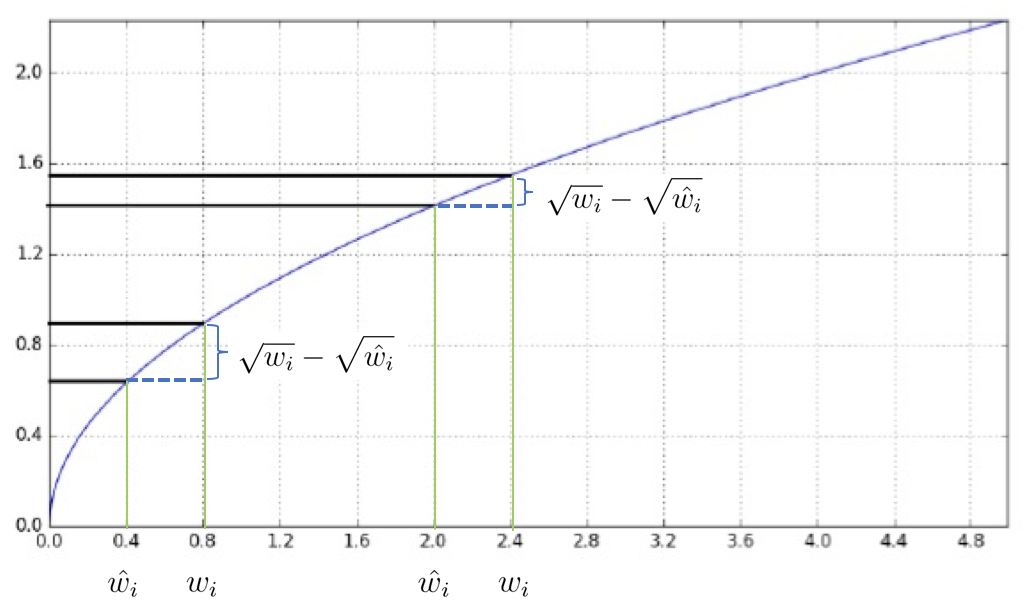
\includegraphics[width=5in]{figures/3_2_检测框尺寸平方根的敏感性曲线}
	\caption{检测框尺寸平方根的敏感性曲线} \label{fig:3_2_检测框尺寸平方根的敏感性曲线}
\end{figure}

前面已经说过,YOLO对每个方格预测多个(默认取B=2)检测框,但在训练时我们只选择与训练数据中物体标记框的IOU最大的检测框来负责该物体的预测,这样使得每个检测框专注于某种特定尺寸、长宽比或物体类型,从而训练出的模型具有更好的预测效果。

至此我们可以给出整个损失函数的数学表达式:
\begin{equation} \label{eq:3_2_loss_function}
\begin{split}
Loss = & \lambda_{coord} \sum_{i=0}^{S^2}\sum_{j=0}^B \mathbf{1}_{ij}^{obj}
			\left[(x_i - \hat{x}_i)^2 + (y_i - \hat{y}_i)^2\right] \\
& + \lambda_{coord}  \sum_{i=0}^{S^2}\sum_{j=0}^B \mathbf{1}_{ij}^{obj}
			\left[ \left(\sqrt{w_i} - \sqrt{\hat{w_i}} \right) ^2 + \left( \sqrt{h_i} - \sqrt{\hat{h_i}} \right) ^2\right] \\
& + \sum_{i=0}^{S^2}\sum_{j=0}^B \mathbf{1}_{ij}^{obj} (C_i - \hat{C_i})^2
			+ \lambda_{noobj} \sum_{i=0}^{S^2}\sum_{j=0}^B \mathbf{1}_{ij}^{noobj} (C_i - \hat{C_i})^2 \\
& + \sum_{i=0}^{S^2} \mathbf{1}_{i}^{obj} \sum_{c \in classes} ( p_i(c) - \hat{p_i}(c) )^2 \\
\end{split}
\end{equation}
式中,当第i个方格中包含待检测的物体时,$\mathbf{1}_{i}^{obj}$取值为1,否则为0;并且只有第i个方格预测的第j个检测框负责该物体的检测时,$\mathbf{1}_{ij}^{obj}$取为1,其余情况都为0。这两个系数的存在确保了只有包含待检测物体的方格会产生对应于物体分类误差的代价项(第四行的代价项,$p(c)$表示该物体属于c类别的概率),以及只有负责检测某个物体的检测框才会产生对应于边界框位置和尺寸误差的代价项(前两行的代价项)。另外需要强调,x、y、w、h分别是相对小方格边长和图像边长归一化后的结果,且x、y的原点是图像中物体所归属方格的左上角。


\subsection{模型改进} % 只写代价函数就不需要单读作为一小节。
% 杨眷玉
(1)代价函数的改进

对于代价函数中的第二项,也就是检测框宽度和高度误差对应的代价项,原算法使用平方根的方式只能在一定程度上改善“相同误差对不同尺寸检测框影响程度不同”这个问题。实际上我们可以利用归一化的思想来对其进行改进:
\begin{equation}
\lambda_{coord}  \sum_{i=0}^{S^2}\sum_{j=0}^B \mathbf{1}_{ij}^{obj}
\left[ \left(\frac{w_i - \hat{w_i}}{w_i} \right) ^2 + \left( \frac{h_i - \hat{h_i}}{h_i} \right) ^2\right]
\end{equation}
通过归一化操作,绝对误差与检测框的尺寸被联系了起来,相当于改为使用检测框尺寸的相对误差来计算代价项,从而解决了存在的问题。

% 《基于双目图像的行人检测与定位系统研究》[J],杨荣坚, ch2.2.1.
(2)分辨率提升 % 注意与实验结果小节的实验参数设置里的cell size统一!

YOLO对待检测的图像施加了非常强的空间约束,因为它将图像划分为7x7的网格,对于方格内的每个检测框最多只能预测单个物体,并且两个检测框只能预测同一类的物体。这种操作导致了YOLO对于相互靠的比较近的物体(比如两个物体的中心落在图像中同一个方格中)以及较小的目标的检测效果不甚理想。为了改善这一状况,我们去掉网络中的最后一个最大池化层,从而网络的输出尺寸变为了14x14,网格的分辨率提升了一倍。这样操作可以在尽量不改变原网络结构的情况下提高模型对相近物体和较小物体的检测能力。


\subsection{网络训练}
根据论文\cite{redmon2016you},YOLO网络需要在ImageNet\cite{russakovsky2015imagenet}包含一千个物体类别的数据集上进行预训练。由于该数据集是用于分类的,预训练时要对网络结构做出一些调整,仅保留前20个卷积层,在之后连接一个平均池化层和一个全连接层以适应分类的任务。预训练完成后,再提出这20个卷积层,连接上文介绍的YOLO网络结构中的后续网络层(即4个卷积层和2个全连接层),使用PASCAL VOC数据集进行训练。进行预训练的操作主要是由于训练数据集的限制。物体检测相关的数据集容量远远小于物体分类使用的数据集,因为其数据标注比较困难,物体分类数据集的标注只是一个类别标签,而对于物体检测,每张图像中可能有一个或多个物体,且需要对每个物体给出一个精确的边界框。PASCAL VOC数据集的图片数量级是$10^4$,这对训练一个二十多层的网络模型是远远不够的;而ImageNet数据集中有1400多万张图片,能够满足网络训练的需求。在ImageNet上训练好20个卷积层的参数后,在PASCAL VOC数据集上主要训练最后4个卷积层和2个全连接层的参数,如图\ref{fig:3_2_网络训练}所示,前20个卷积层的参数不会再发生显著的改变。为了加快预训练的速度,预训练时网络输入的尺寸设置为224*224;而正式训练时为了获得更高的检测精度,改用较高的图像分辨率,网络输入尺寸被设置为448*448。

\begin{figure}[htb] %YOLO网络训练
	\centering
	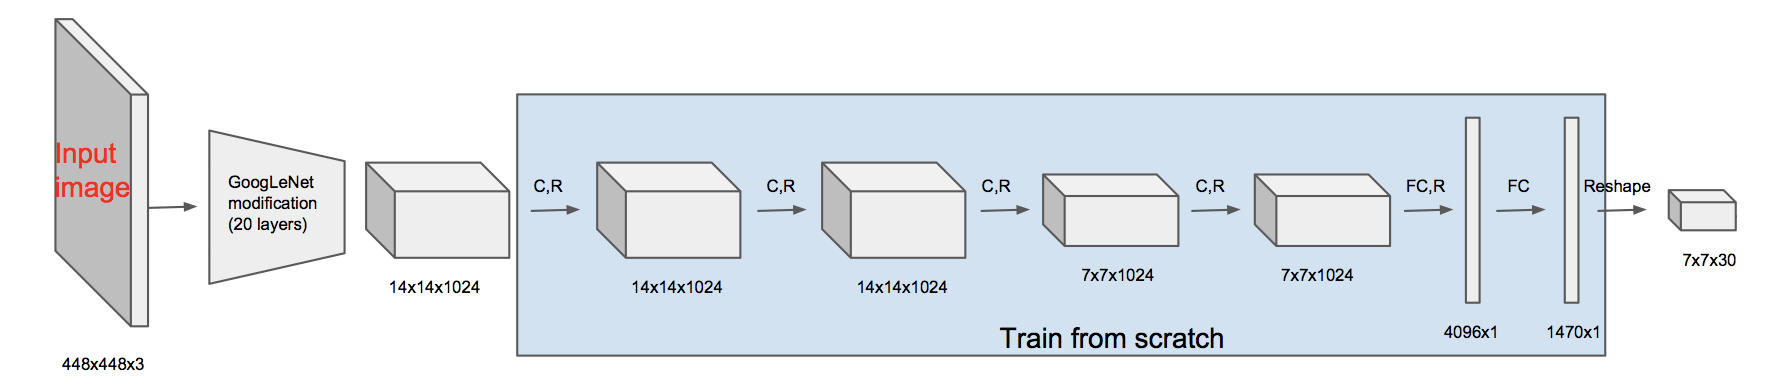
\includegraphics[width=6.5in]{figures/3_2_网络训练}
	\caption{YOLO网络训练} \label{fig:3_2_网络训练}
\end{figure}

% 这段放在{网络训练}还是{实验结果}?
网络的预训练需要大约一周的时间,且ImageNet数据集需占用约1T的硬盘空间。由于GPU运算资源、存储空间和时间的限制,本文的实验直接使用网络上提供的预训练结果在PASCAL VOC训练数据集上进行训练。

% pascal voc数据集介绍要不要紧跟上段?


% 数据预处理?归一化
训练使用的图像在输入网络时需先进行归一化处理,将像素值压缩到[-1, 1]区间内:
\begin{equation}
I(x, y) = \frac{I(x, y)}{255.0} * 2.0 - 1.0
\end{equation}

% 数据增强
另外进行了一些数据增强(data augmentation)操作,以增大训练数据量,减少过拟合,从而获得更好的模型泛化效果。
具体操作可选择图像尺寸变换(resize)、图像水平翻转(horizontal flip)、图像白化(whiten)、图像切割(crop)、添加高斯噪声、对比度变换和颜色变换等。对于尺寸变换、水平翻转和图像切割操作,需对图像对应的标签文件进行修改,以保证检测框的坐标与变换后的图像一致。

尺寸变换可根据下式来计算随机的图像宽高比new\_ar和缩放因子scale。w和h是输入图像的宽度和高度,randint()生成两个参数范围内的随机整数,random()生成0到1之间的随机数,$\alpha$为可调整的参数,实验中取0.2。
% yolo-tf_persistforever/src/data/image_mp_v2.py
\begin{align} %aspect ratio
new\_ar &= \frac{w + randint(-w*\alpha, w*\alpha)}{h + randint(-h*\alpha, h*\alpha)} \\
scale &= random() * 0.4 + 0.8
\end{align}

正式训练采用加入动量项的小批量随机梯度下降算法(mini-batch stochastic gradient descent)优化器,动量系数取0.9,并在对训练参数应用了指数衰减的滑动平均(exponential moving average),衰减因子取0.9999。

%------------------------------------------------------------------------------------
\section{实验结果}
% YOLO_small.ckpt并不是预训练的结果啊。而是训练完成的结果了。那还finetune个屁啊,图敢不敢贴?

\subsection{PASCAL VOC数据集}
% 数据集具体介绍。文件夹结构,xml文件内容?
PASCAL VOC数据集来源于2005年到2012年间举办的物体分类识别和检测挑战赛。目前流行使用的是2007年和2012年的数据集,因为在2007年数据集首次扩大到20个类别,而2012年的数据集包含了2008到2011年的所有图片。

PASCAL VOC数据集的20个类别可以分为四个大类:人类、7种日常使用的交通工具(火车、轿车、公共汽车、摩托车、自行车、船只和飞机)、6种动物(牛、羊、马、猫、狗和鸟类)以及6种室内常见家具或物品(餐桌、椅子、盆栽植物、沙发、瓶子和电视或显示器)。数据集分为训练集、验证集和测试集,2007版合计9963张图片,内含24640个带有具体标记数据的物体;2012版合计17125张图片,内含27450个带标记的物体。每张图片对应的xml文件内包含物体检测任务所需的物体类别、边界框的位置和尺寸信息。该数据集图像质量好,内容丰富,标注完整,非常适合用于相关模型的训练和算法的测试。
本实验使用PASCAL VOC 2007和2012的训练数据进行模型训练,使用2007版的测试数据进行模型测试。
% 先这么写吧。。只用2007训练效果肯定更差。。
% 此处可以加图。图片样本如图...所示。

\subsection{实验环境及训练平台}
本实验使用的计算机配置见表\ref{tab:3_3_experiment_environment}。
\begin{table}[htbp]
	\centering
	\caption{实验运行环境} \label{tab:3_3_experiment_environment}
	\begin{small} %{scriptsize}
		\begin{tabular}{|c|c|}\hline
			项目  & 配置参数  \\\hline
			%---------------------------------------------------------
			CPU & Intel(R) Xeon(R) CPU E5-2630 v2 @2.60GHz, 12核 \\
			内存 & 24G \\
			显卡 & NVidia GeForce GTX TITAN X \\
			显存 & 12G \\
			CUDA & V7.5 \\
			操作系统 & Ubuntu 16.04.1 LTS \\\hline
		\end{tabular}
	\end{small} %{scriptsize}
\end{table}

% tensorflow介绍。
网络模型的搭建、训练与测试使用开源深度学习平台TensorFlow\cite{abadi2016tensorflow}。
TensorFlow是谷歌开发的第二代人工智能学习平台,前身是DistBelief,主要应用于深度学习领域。其采用数据流图(data flow graph)的形式来建立模型,图中每个节点表示一个数学运算或数据的输入/输出,每条边则表示节点间的输入输出关系,边上传输的是多维数组数据,即张量(Tensor)。模型的计算过程就是张量在数据流图中的流动过程,这种设计思路使其具有高度的灵活性,可以通过组装现有模块或定义新的操作来搭建自己所需的模型。

TensorFlow具有自动求微分的功能,非常适合于深度神经网络这类基于梯度的机器学习算法。对于其他类型的机器学习算法,TensorFlow同样能够胜任,只要能够将计算表示为数据流图的形式就可以解决。另外,TensorFlow具有高度的可移植性,可以在台式机、服务器和移动设备的CPU或GPU上运行,也能够较容易地实现分布式的部署。

\subsection{实验参数设置}
实验使用的模型参数、训练和测试参数取值见表\ref{tab:3_3_params}。
\begin{table}[htbp]
	\centering
	\caption{实验参数设置} \label{tab:3_3_params}
	\begin{small} %{scriptsize}
		\begin{tabular}{|c|c|c|c|c|c|}\hline
			模型参数                   & 取值  & 训练参数              & 取值       & 测试参数   & 取值 \\\hline
			%---------------------------------------------------------
			IMAGE\_SIZE            & 448   &  LEARNING\_RATE & 0.0001   & THRESHOLD & 0.2 \\
			CELL\_SIZE               & 14     &  DECAY\_STEPS     & 30000    & IOU\_THRESHOLD & 0.5 \\
			% TODO: 注意CELL_SIZE与上一小节模型改进中提高分辨率操作后一致
			BOX\_PER\_CELL       & 2       &  DECAY\_RATE      & 0.1         & & \\
			$\lambda_{obj}$        & 1       &  BATCH\_SIZE       & 45          & & \\
			$\lambda_{noobj}$    & 0.5    &  MAX\_ITER           & 30000    & & \\
			%TODO:MAX_ITER写1w5还是3w? 不贴图就写3w吧。
			$\lambda_{class}$     & 2       &  SUMMARY\_ITER  & 10         &  & \\
			$\lambda_{coord}$    & 5       & SAVE\_ITER           & 1000      &  & \\\hline
		\end{tabular}
	\end{small} %{scriptsize}
\end{table}

\subsection{实验结果与分析}
图\ref{fig:3_3_测试结果}展示了模型训练完成后在PASCAL VOC 2007测试集上部分图片的检测效果。 考虑到本文算法实际应用时以旋翼无人机为载体,应用场景主要为室外,因此选择的都是室外包含人、交通工具、动物等目标的图片。
测试结果显示YOLO目标检测模型具有优秀的检测能力。由于在训练和检测的过程中利用了整张图像的全局信息,相较基于区域提名(region proposal)的算法,其将背景错误归为物体的概率要低很多。
\begin{figure}[htbp] %测试结果
	\centering
	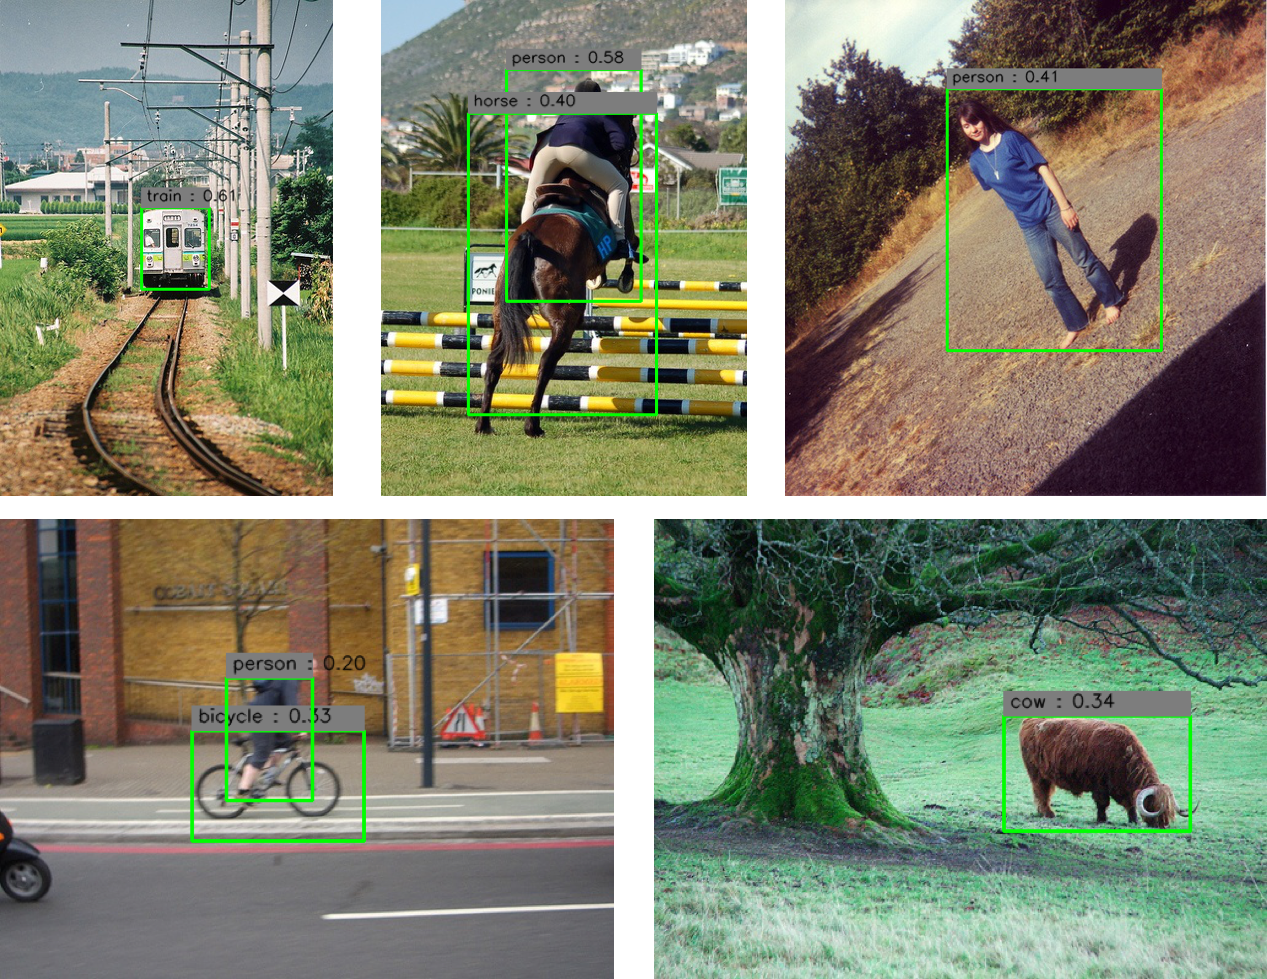
\includegraphics[width=6in]{figures/3_3_voc2007_test_result1}\vspace{.1in}
	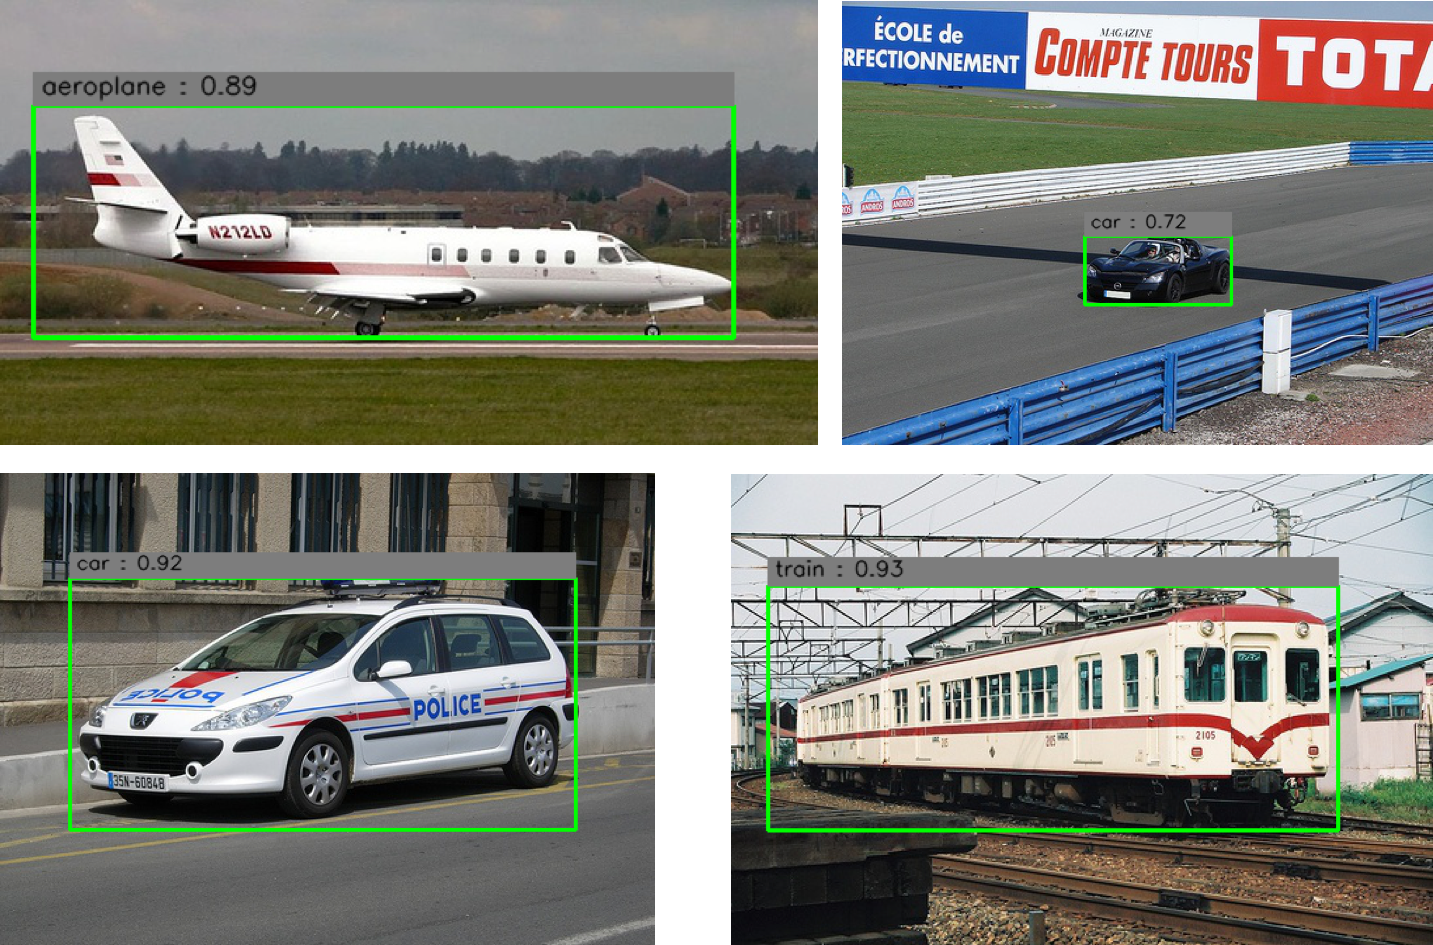
\includegraphics[width=6in]{figures/3_3_voc2007_test_result2}
	\caption{YOLO在PASCAL VOC 2007测试集上的部分测试结果}\label{fig:3_3_测试结果}
\end{figure}

YOLO的最大优点在于运行速度。基于前文介绍的计算机配置,在GPU上每张图片的处理时间为0.031s,即32Hz;在CPU上每张图片的处理时间约为0.35s。在使用GPU计算时,有一些图像的预处理(尺寸变化、像素值归一化等)是在CPU上使用python的cv2和numpy等模块完成的,若将这些运算转移到GPU上进行,则程序的运行速度还能获得一定的提升。实时检测效果如图\ref{fig:3_3_实时检测效果}所示。
\begin{figure}[htbp] %实时检测效果
	\centering
	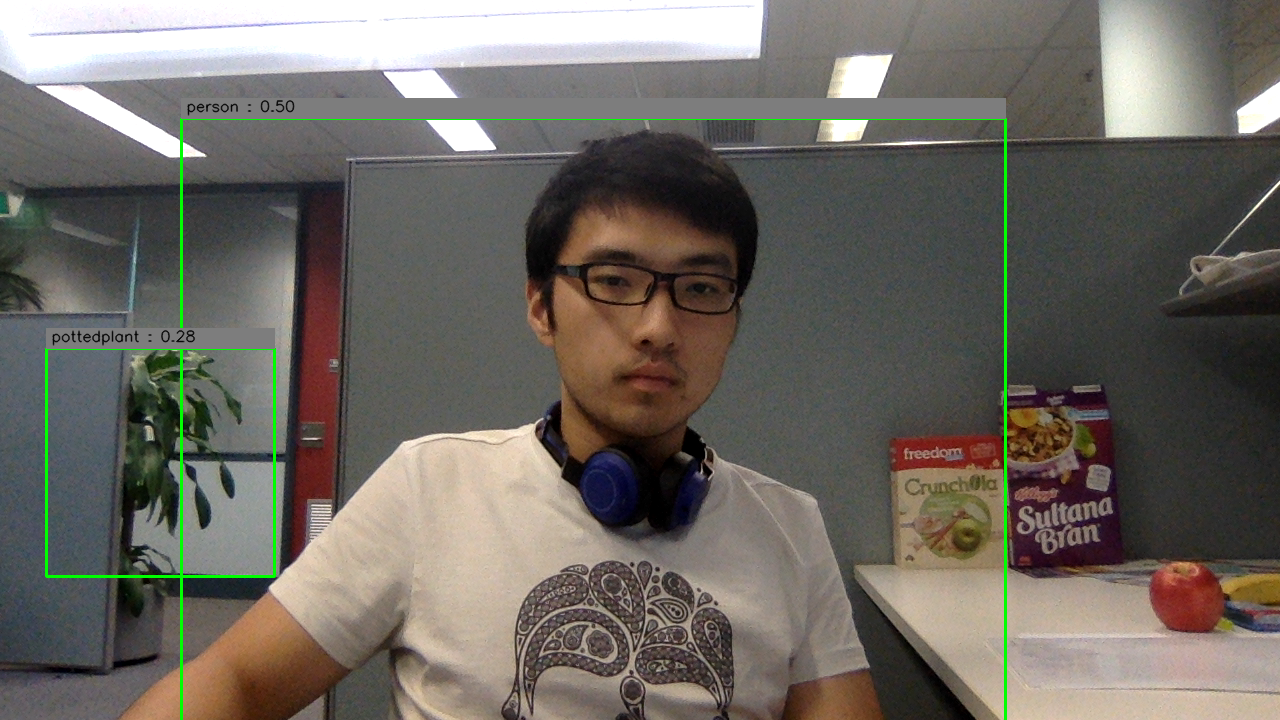
\includegraphics[width=3.5in]{figures/3_3_realtime_detection}
	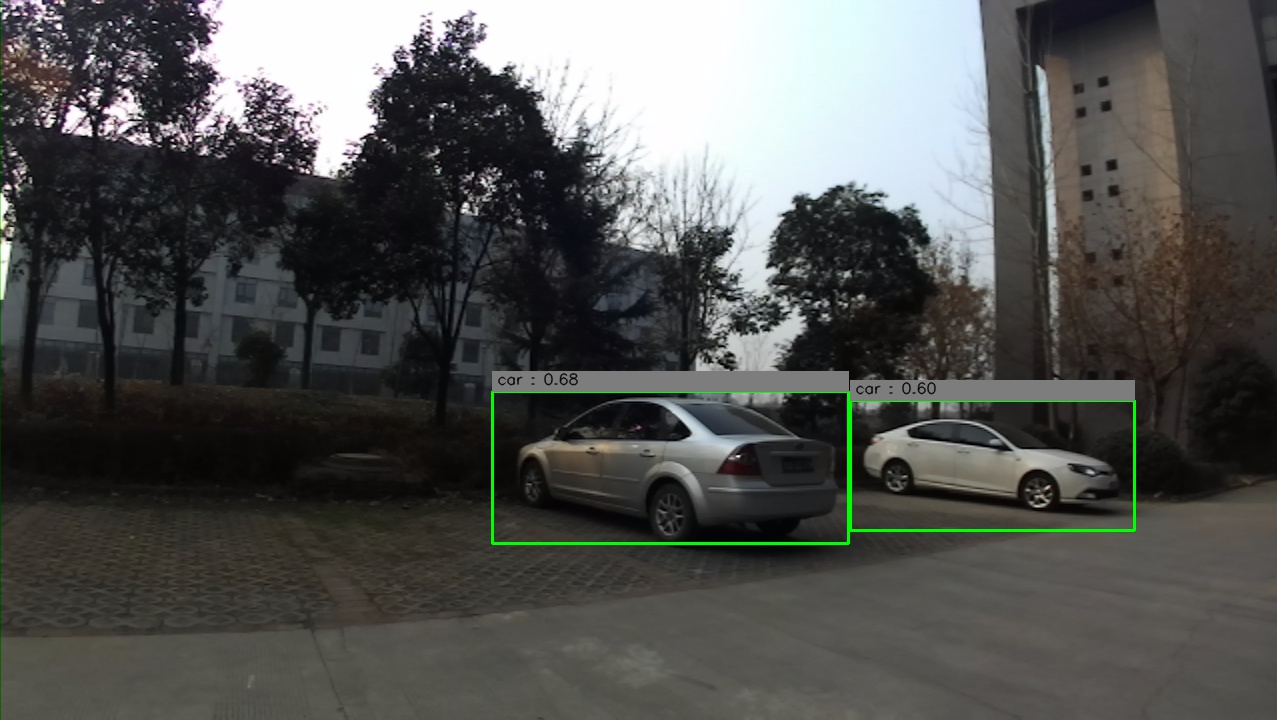
\includegraphics[width=3.5in]{figures/3_3_realtime_detection2}
	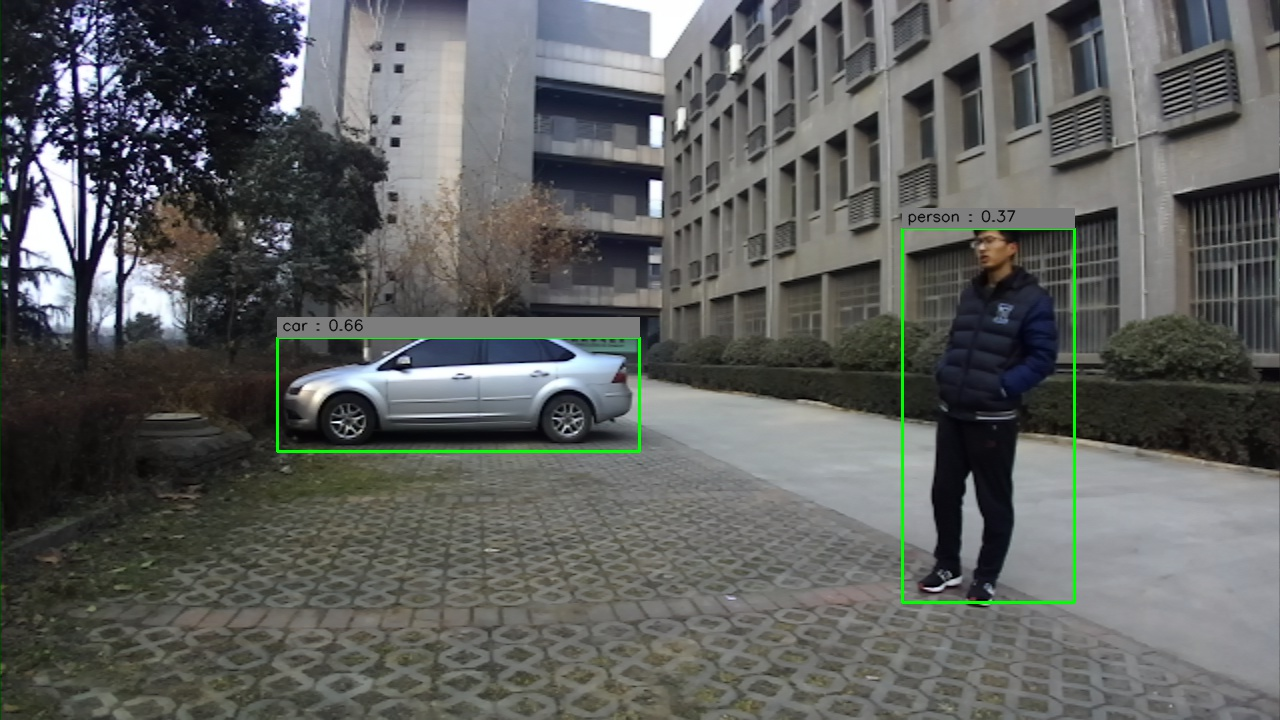
\includegraphics[width=3.5in]{figures/3_3_realtime_detection3}
	\caption{YOLO实时检测效果}\label{fig:3_3_实时检测效果}
\end{figure}

% 缺点
% 小物体、靠近的物体;不常见的长宽比;定位误差大。基于IOU的NMS也有问题(一个bbox包含另一个时)。
在测试中,我们也发现了一些效果不佳的测试图片,如图\ref{fig:3_3_反面结果}。根据文献和实验结果,可以总结出算法的主要缺点。
由于检测框是基于网格的,其对于局部聚集和堆叠的物体检测效果不佳。通过提高分割网格的分辨率可以在一定程度上改善这种状况,但无法从本质上解决问题。
当图像的宽高比偏离1较多时,检测效果会逐渐变差。这是因为图片输入网络时都需要变换到固定尺寸,而过大的宽高比变化会导致物体严重变形,从而检测结果中的检测框精度会变差,甚至直接检测失败。
%%这条要写吗?%突然觉得增大网格分辨率可能导致结果中有更多未被剔除的bbox。
%另外,基于IOU阈值的NMS有时也会出现问题,比如当一个较大的检测框包含一个较小的检测框且其IOU低于阈值时,就无法被剔除。
YOLO的定位误差相较Faster R-CNN等算法更大,而对于本文使用双目摄像机拍摄的图片,在前景背景分明的情况下我们可以利用深度信息对检测框的位置进行调整,以获得更精确的定位结果。
\begin{figure}[htbp] %反面结果。该不该贴?。。
	\centering
	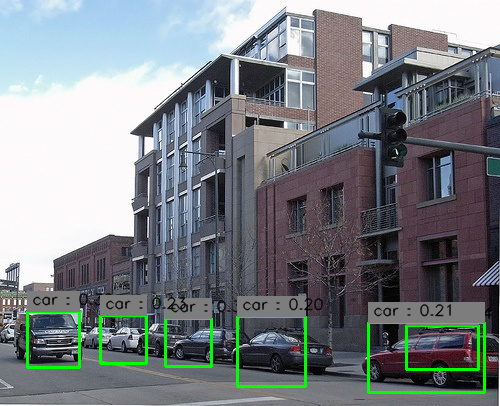
\includegraphics[width=2.5in]{figures/3_3_反面结果1} % 这张比较高,缩小一点
	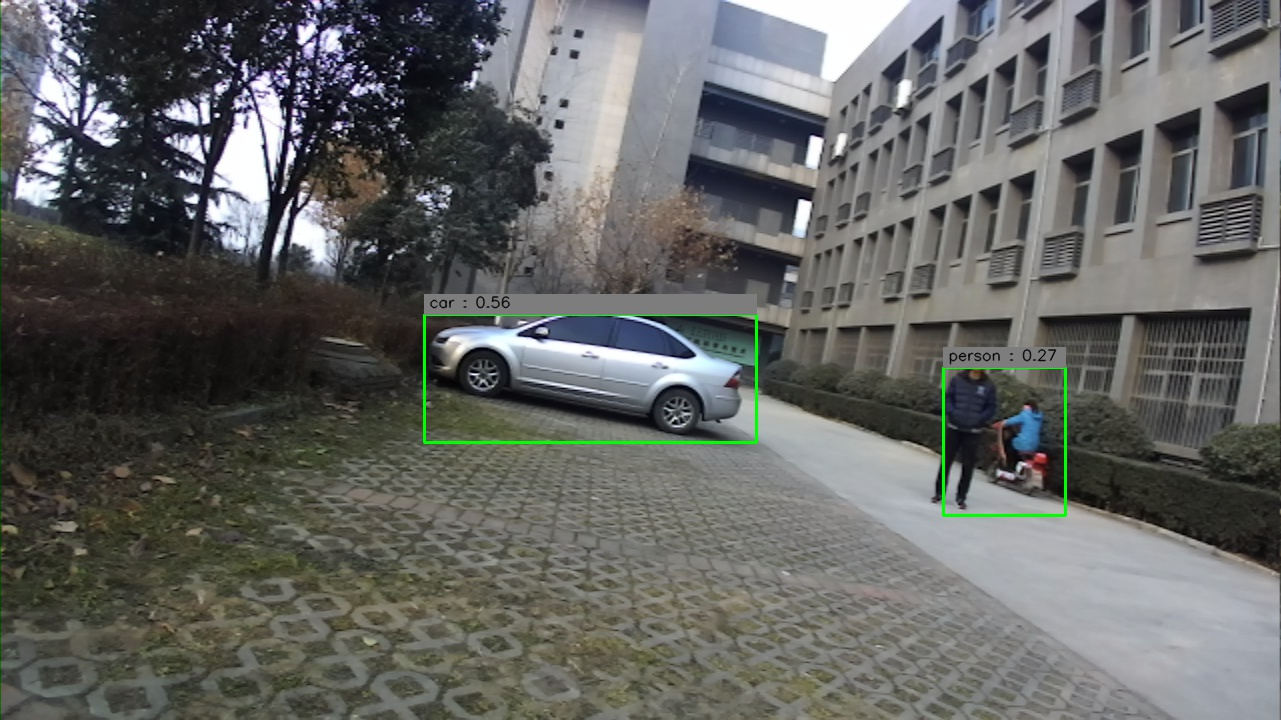
\includegraphics[width=3.5in]{figures/3_3_反面结果2}
	\caption{效果不佳的检测结果}\label{fig:3_3_反面结果}
\end{figure}


% 定量的结果。be honest, or make up something?
由于本文使用目标检测主要出于为基于立体视觉的目标定位设定定位目标的目的,目前暂未进行定量的平均检测准确度(mAP)的统计。平均检测准确度、检准率(Precision)和召回率(Recall,也叫查全率)是评价目标检测算法的重要指标,我们将算法的定量测试结果和与其他算法的比较列入后续工作。
%(map什么的要介绍吗?)
% 本文进统计了目标为行人/车辆的查准率、查全率。《基于YOLO算法的车辆实时检测》


%------------------------------------------------------------------------------------
\section{本章小结}
本章主要介绍了基于卷积神经网络的YOLO目标检测系统。首先介绍了卷积神经网络的相关理论知识,包括卷积运算的三个基本思想(稀疏连接、参数共享和等变表示)、CNN的结构以及模型训练中的反向传播和梯度下降算法。之后引入YOLO目标检测模型,分析了其检测策略和过程,介绍了网络结构与损失函数的定义,并针对存在的问题提出了改进方案。使用TensorFlow平台搭建了网络模型并在PASCAL VOC数据集上进行了训练,最后给出了实验结果并分析了算法的优缺点。测试结果显示,实验中训练的模型具有较好的检测效果以及出色的实时性能。





